\documentclass{standalone}
\usepackage{tikz}
\usetikzlibrary{patterns, positioning}

\begin{document}
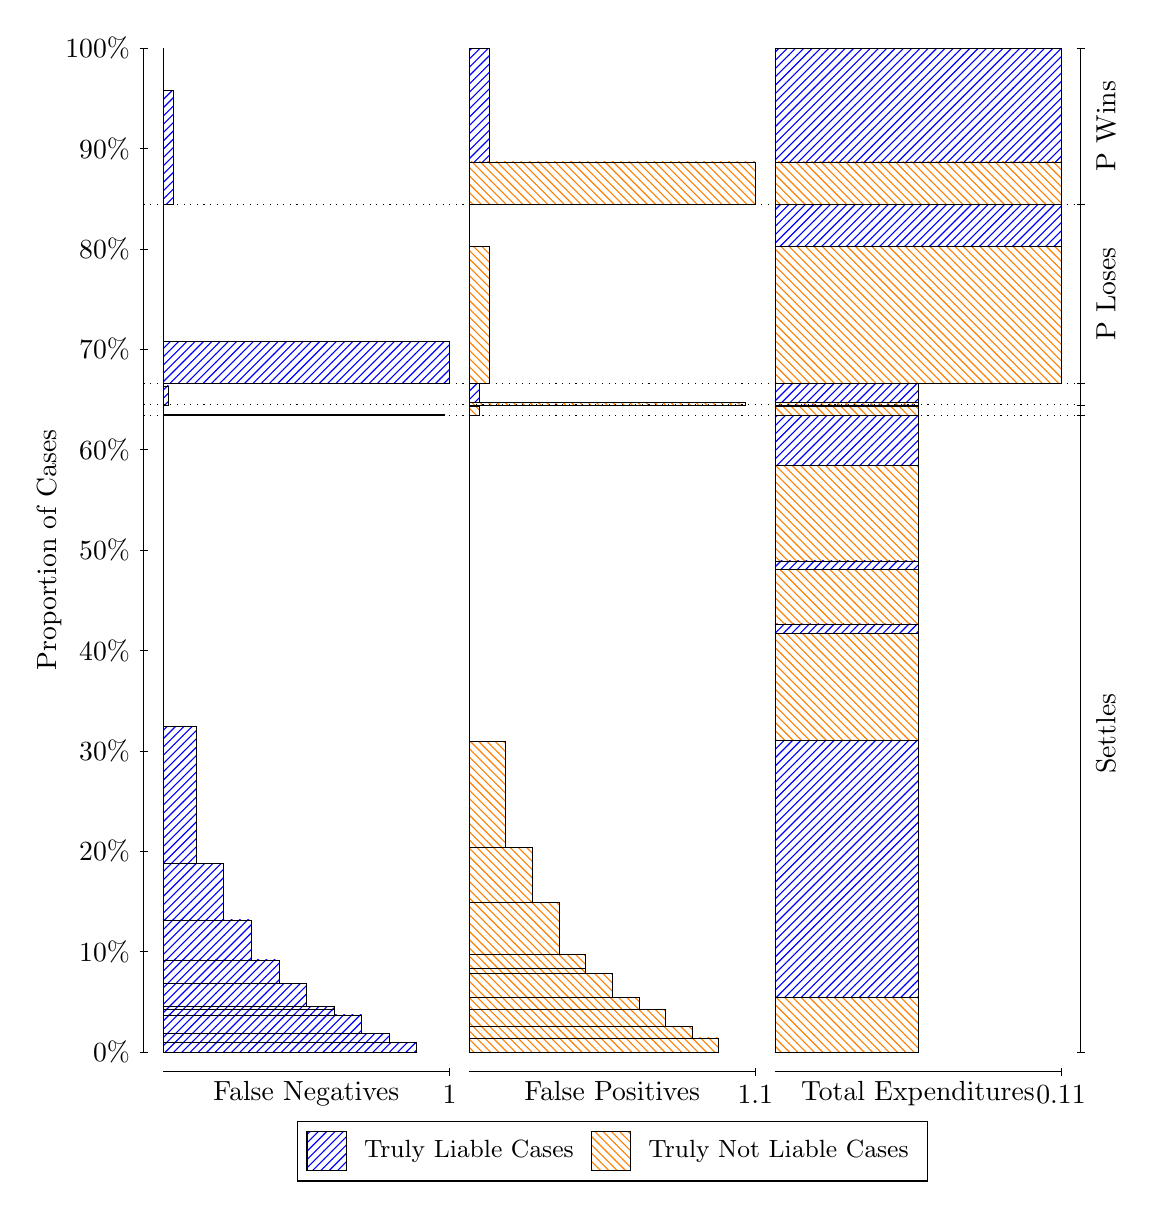
\begin{tikzpicture}
\draw[black, very thin] (1.5,1.75) -- (1.5,14.5);
\node[rotate=90, anchor=center] at (0.3, 8.125) {Proportion of Cases};
\draw[black, very thin] (1.45,1.75) -- (1.55,1.75);
\node[anchor=east] at (1.45, 1.75) {0\%};
\draw[black, very thin] (1.45,3.025) -- (1.55,3.025);
\node[anchor=east] at (1.45, 3.025) {10\%};
\draw[black, very thin] (1.45,4.3) -- (1.55,4.3);
\node[anchor=east] at (1.45, 4.3) {20\%};
\draw[black, very thin] (1.45,5.575) -- (1.55,5.575);
\node[anchor=east] at (1.45, 5.575) {30\%};
\draw[black, very thin] (1.45,6.85) -- (1.55,6.85);
\node[anchor=east] at (1.45, 6.85) {40\%};
\draw[black, very thin] (1.45,8.125) -- (1.55,8.125);
\node[anchor=east] at (1.45, 8.125) {50\%};
\draw[black, very thin] (1.45,9.4) -- (1.55,9.4);
\node[anchor=east] at (1.45, 9.4) {60\%};
\draw[black, very thin] (1.45,10.675) -- (1.55,10.675);
\node[anchor=east] at (1.45, 10.675) {70\%};
\draw[black, very thin] (1.45,11.95) -- (1.55,11.95);
\node[anchor=east] at (1.45, 11.95) {80\%};
\draw[black, very thin] (1.45,13.225) -- (1.55,13.225);
\node[anchor=east] at (1.45, 13.225) {90\%};
\draw[black, very thin] (1.45,14.5) -- (1.55,14.5);
\node[anchor=east] at (1.45, 14.5) {100\%};

\draw[black, very thin] (13.4,1.75) -- (13.4,14.5);
\draw[black, very thin] (13.35,1.75) -- (13.45,1.75);
\node[anchor=west] at (13.35, 1.75) {};
\draw[black, very thin] (13.35,9.8345) -- (13.45,9.8345);
\node[anchor=west] at (13.35, 9.8345) {};
\draw[black, very thin] (13.35,9.9675) -- (13.45,9.9675);
\node[anchor=west] at (13.35, 9.9675) {};
\draw[black, very thin] (13.35,10.24) -- (13.45,10.24);
\node[anchor=west] at (13.35, 10.24) {};
\draw[black, very thin] (13.35,12.517) -- (13.45,12.517);
\node[anchor=west] at (13.35, 12.517) {};
\draw[black, very thin] (13.35,14.5) -- (13.45,14.5);
\node[anchor=west] at (13.35, 14.5) {};

\draw[black, very thin, pattern color=blue, pattern=north east lines] (1.75,1.75) rectangle (4.9675,1.8744);
\draw[black, very thin, pattern color=blue, pattern=north east lines] (1.75,1.8744) rectangle (4.6173,1.9838);
\draw[black, very thin, pattern color=blue, pattern=north east lines] (1.75,1.9838) rectangle (4.2671,2.2213);
\draw[black, very thin, pattern color=blue, pattern=north east lines] (1.75,2.2213) rectangle (3.9169,2.2888);
\draw[black, very thin, pattern color=blue, pattern=north east lines] (1.75,2.2888) rectangle (3.9169,2.3311);
\draw[black, very thin, pattern color=blue, pattern=north east lines] (1.75,2.3311) rectangle (3.5667,2.6184);
\draw[black, very thin, pattern color=blue, pattern=north east lines] (1.75,2.6184) rectangle (3.2165,2.9196);
\draw[black, very thin, pattern color=blue, pattern=north east lines] (1.75,2.9196) rectangle (2.8663,3.4281);
\draw[black, very thin, pattern color=blue, pattern=north east lines] (1.75,3.4281) rectangle (2.5161,4.1469);
\draw[black, very thin, pattern color=blue, pattern=north east lines] (1.75,4.1469) rectangle (2.1659,5.8868);
\draw[black, very thin, pattern color=orange, pattern=north west lines] (1.75,5.8868) rectangle (1.75,9.8345);
\draw[black, very thin, pattern color=blue, pattern=north east lines] (1.75,9.8345) rectangle (5.3177,9.8463);
\draw[black, very thin, pattern color=orange, pattern=north west lines] (1.75,9.8463) rectangle (1.75,9.9675);
\draw[black, very thin, pattern color=blue, pattern=north east lines] (1.75,9.9675) rectangle (1.8157,10.21);
\draw[black, very thin, pattern color=orange, pattern=north west lines] (1.75,10.21) rectangle (1.75,10.24);
\draw[black, very thin, pattern color=blue, pattern=north east lines] (1.75,10.24) rectangle (5.3833,10.777);
\draw[black, very thin, pattern color=orange, pattern=north west lines] (1.75,10.777) rectangle (1.75,12.517);
\draw[black, very thin, pattern color=blue, pattern=north east lines] (1.75,12.517) rectangle (1.8813,13.965);
\draw[black, very thin, pattern color=orange, pattern=north west lines] (1.75,13.965) rectangle (1.75,14.5);
\draw[black, very thin, pattern color=orange, pattern=north west lines] (5.6333,1.75) rectangle (8.8019,1.9295);
\draw[black, very thin, pattern color=orange, pattern=north west lines] (5.6333,1.9295) rectangle (8.464,2.0704);
\draw[black, very thin, pattern color=orange, pattern=north west lines] (5.6333,2.0704) rectangle (8.126,2.2886);
\draw[black, very thin, pattern color=orange, pattern=north west lines] (5.6333,2.2886) rectangle (7.788,2.44);
\draw[black, very thin, pattern color=orange, pattern=north west lines] (5.6333,2.44) rectangle (7.45,2.7503);
\draw[black, very thin, pattern color=orange, pattern=north west lines] (5.6333,2.7503) rectangle (7.112,2.8095);
\draw[black, very thin, pattern color=orange, pattern=north west lines] (5.6333,2.8095) rectangle (7.112,2.9921);
\draw[black, very thin, pattern color=orange, pattern=north west lines] (5.6333,2.9921) rectangle (6.774,3.6544);
\draw[black, very thin, pattern color=orange, pattern=north west lines] (5.6333,3.6544) rectangle (6.436,4.3437);
\draw[black, very thin, pattern color=orange, pattern=north west lines] (5.6333,4.3437) rectangle (6.0981,5.6978);
\draw[black, very thin, pattern color=blue, pattern=north east lines] (5.6333,5.6978) rectangle (5.6333,9.8345);
\draw[black, very thin, pattern color=orange, pattern=north west lines] (5.6333,9.8345) rectangle (5.7601,9.9558);
\draw[black, very thin, pattern color=blue, pattern=north east lines] (5.6333,9.9558) rectangle (5.6333,9.9675);
\draw[black, very thin, pattern color=orange, pattern=north west lines] (5.6333,9.9675) rectangle (9.1399,9.998);
\draw[black, very thin, pattern color=blue, pattern=north east lines] (5.6333,9.998) rectangle (5.7601,10.24);
\draw[black, very thin, pattern color=orange, pattern=north west lines] (5.6333,10.24) rectangle (5.8868,11.981);
\draw[black, very thin, pattern color=blue, pattern=north east lines] (5.6333,11.981) rectangle (5.6333,12.517);
\draw[black, very thin, pattern color=orange, pattern=north west lines] (5.6333,12.517) rectangle (9.2667,13.053);
\draw[black, very thin, pattern color=blue, pattern=north east lines] (5.6333,13.053) rectangle (5.8868,14.5);
\draw[black, very thin, pattern color=orange, pattern=north west lines] (9.5167,1.75) rectangle (11.333,2.44);
\draw[black, very thin, pattern color=blue, pattern=north east lines] (9.5167,2.44) rectangle (11.333,5.7084);
\draw[black, very thin, pattern color=orange, pattern=north west lines] (9.5167,5.7084) rectangle (11.333,7.0624);
\draw[black, very thin, pattern color=blue, pattern=north east lines] (9.5167,7.0624) rectangle (11.333,7.1868);
\draw[black, very thin, pattern color=orange, pattern=north west lines] (9.5167,7.1868) rectangle (11.333,7.8761);
\draw[black, very thin, pattern color=blue, pattern=north east lines] (9.5167,7.8761) rectangle (11.333,7.9854);
\draw[black, very thin, pattern color=orange, pattern=north west lines] (9.5167,7.9854) rectangle (11.333,9.1999);
\draw[black, very thin, pattern color=blue, pattern=north east lines] (9.5167,9.1999) rectangle (11.333,9.8345);
\draw[black, very thin, pattern color=orange, pattern=north west lines] (9.5167,9.8345) rectangle (11.333,9.9558);
\draw[black, very thin, pattern color=blue, pattern=north east lines] (9.5167,9.9558) rectangle (11.333,9.9675);
\draw[black, very thin, pattern color=orange, pattern=north west lines] (9.5167,9.9675) rectangle (11.333,9.998);
\draw[black, very thin, pattern color=blue, pattern=north east lines] (9.5167,9.998) rectangle (11.333,10.24);
\draw[black, very thin, pattern color=orange, pattern=north west lines] (9.5167,10.24) rectangle (13.15,11.981);
\draw[black, very thin, pattern color=blue, pattern=north east lines] (9.5167,11.981) rectangle (13.15,12.517);
\draw[black, very thin, pattern color=orange, pattern=north west lines] (9.5167,12.517) rectangle (13.15,13.053);
\draw[black, very thin, pattern color=blue, pattern=north east lines] (9.5167,13.053) rectangle (13.15,14.5);
\draw[black, dotted] (1.5,9.8345) -- (13.4,9.8345);
\draw[black, dotted] (1.5,9.9675) -- (13.4,9.9675);
\draw[black, dotted] (1.5,10.24) -- (13.4,10.24);
\draw[black, dotted] (1.5,12.517) -- (13.4,12.517);
\draw[black, very thin] (1.75,1.5) -- (5.3833,1.5);
\node[anchor=north] at (3.5667, 1.5) {False Negatives};
\draw[black, very thin] (5.3833,1.45) -- (5.3833,1.55);
\node[anchor=north] at (5.3833, 1.45) {1};

\draw[black, very thin] (5.6333,1.5) -- (9.2667,1.5);
\node[anchor=north] at (7.45, 1.5) {False Positives};
\draw[black, very thin] (9.2667,1.45) -- (9.2667,1.55);
\node[anchor=north] at (9.2667, 1.45) {1.1};

\draw[black, very thin] (9.5167,1.5) -- (13.15,1.5);
\node[anchor=north] at (11.333, 1.5) {Total Expenditures};
\draw[black, very thin] (13.15,1.45) -- (13.15,1.55);
\node[anchor=north] at (13.15, 1.45) {0.11};

\node[black, centered, rotate=90] at (13.72, 5.7923) {Settles};


\node[black, centered, rotate=90] at (13.72, 11.379) {P Loses};
\node[black, centered, rotate=90] at (13.72, 13.509) {P Wins};

\draw (7.449999999999999,1.5) node[draw=none] (baseCoordinate) {};
\begin{scope}[align=center]
        \matrix[scale=0.5, draw=black, below=0.5cm of baseCoordinate, nodes={draw}, column sep=0.1cm]{
            \node[rectangle, draw, minimum width=0.5cm, minimum height=0.5cm, pattern=north east lines, pattern color=blue] {}; &
            \node[draw=none, font=\small] (B) {Truly Liable Cases}; &
            \node[rectangle, draw, minimum width=0.5cm, minimum height=0.5cm, pattern=north west lines, pattern color=orange] {}; &
            \node[draw=none, font=\small] (B) {Truly Not Liable Cases}; \\
            };
\end{scope}

\end{tikzpicture}
\end{document}